\documentclass{IEEEtran}
\usepackage{amsfonts}
\usepackage{amsmath}
\usepackage{amsthm}
\usepackage{amssymb}
\usepackage{enumitem}
\usepackage{xcolor}
\usepackage{graphicx}
\usepackage{caption}
\usepackage{csquotes}
\usepackage{fontawesome}
\usepackage{hyperref}

\newcommand{\aaa}[2]
	{\href{#1}{#2}}

\title{KWS2102 Term 1 Report: Sobel Operator VHDL Implementation (Repo: \aaa{https://github.com/slypiggies/fyp}{\faGithub})}
\author{Lam Kin Long (1155127407)}

\begin{document}
	\maketitle
	\begin{abstract}
		In this paper, a field-programmable gate array (FPGA) system for edge detection has been developed. This system allows in real-time, finding edges from a live video stream in VGA 640x480 resolution. Edges of objects with distinct background colors are highlighted in white. The system uses the Xilinx ZedBoard with the XC7Z020 system on a chip (SoC) as the main processing unit, a single camera sensor OV7670 for video acquisition, and VGA \cite{vga} for video output. The system is coded in the hardware description language (HDL) VHDL, developed on the Xilinx Vivado software suite, and lays out the foundation for future object detection work. Possibilities include detection of QR codes and AprilTags.
	\end{abstract}
	\section{Introduction}
	One of the most challenging problems which robots face is how they can align themselves with the outside world. If the robots are not controlled manually, they will need to use sensors to perceive ambient parameters. Unless the terrains are specifically designed for the robots, they cannot rely on primitive techniques like tracing black lines. While humans can simply use their eyes to locate where they are, robots need specialized 2D codes, realistically recognized within a very short and bounded amount of time, known as real-time. For AprilTags, the first step of code detection involves edge detection. For other 2D codes such as QR codes and DataMatrices, the first steps may differ. Regardless, edge detection is a highly relevant yet fundamental problem, which is good for setting up the overall system and for me to be familiar with FPGAs and VHDL.
	\begin{figure}[h]
		\centering
		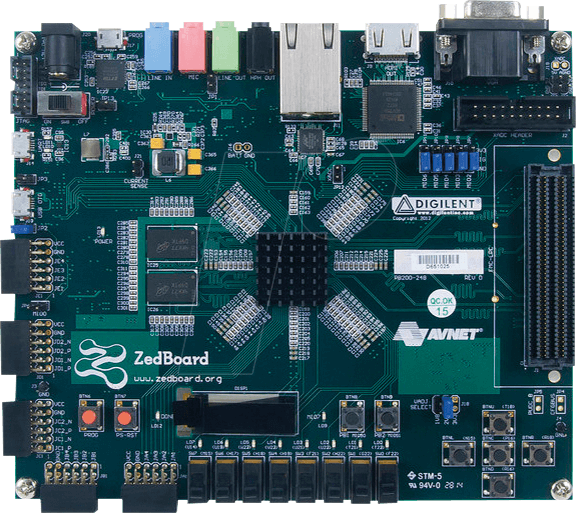
\includegraphics[scale=0.33]{zedboard}
		\caption{Xilinx ZedBoard}
		\label{fig:zedboard}
	\end{figure}
	FPGA is chosen for the task because of its large amount of I/O. It is also inherently good at achieving deep pipelining. Large parallelism can also be achieved on an FPGA, if it is being programmed explicitly to do so. Compared to application-specific integrated circuit (ASIC), FPGA is better for prototyping because of it being reconfigurable. ASIC is fixed, very expensive to manufacture, even though it can be more efficient than an FPGA. ASIC is typically for designs that have already been tested with FPGAs.
	
	Two other obvious alternatives include microcontrollers (MCU) and single-board computers (SBC). The on-board oscillator of a popular MCU, Arduino Uno, can only go up to 16 MHz, which is slower than just the pixel clock from the camera. It also only has 22 available pins, which assuming can all be used simultaneously, are still barely enough for the current system \footnote{16 pins for the camera, 5 pins for VGA (3 of them, RGB, being analog), 1 pin for reset, excluding any power and ground pins}. More powerful MCUs may be suitable for the current system’s application, but they leave little room for future expansions, compared to FPGAs. For SBCs, online demo shows that a Raspberry Pi 3B+ can process only up to 10 FPS \cite{rpi}, just by doing edge detection alone. Moreover, most SBCs run Linux, instead of a real-time operating system, and in theory the response time cannot be guaranteed. Unless more power-hungry and expensive computers with dedicated graphics are considered, FPGA is the better choice.
	\begin{figure}[h]
		\centering
		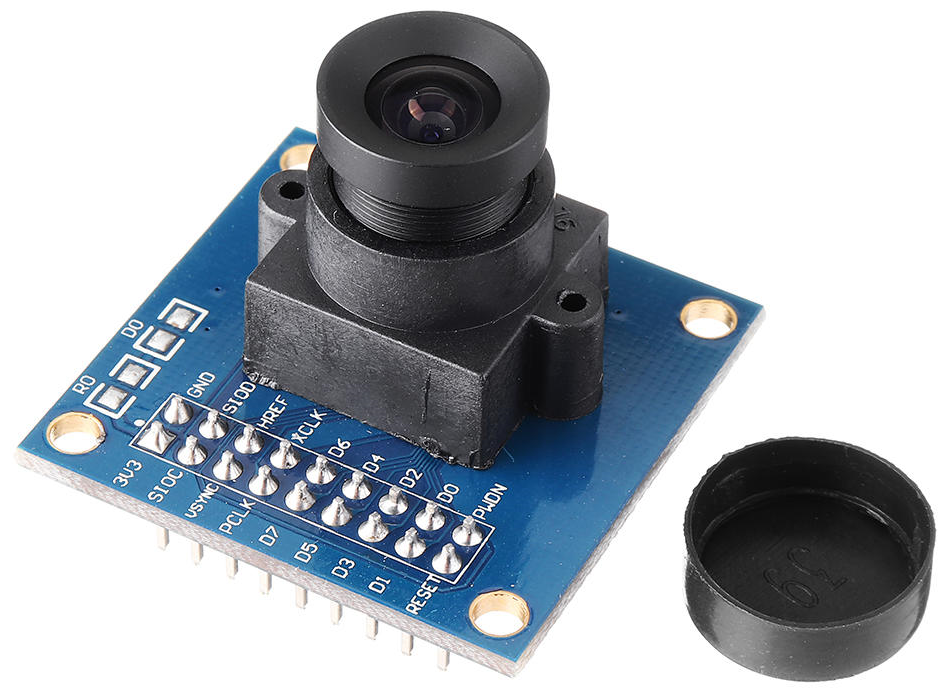
\includegraphics[scale=0.1]{ov7670}
		\caption{OmniVision OV7670}
		\label{fig:ov7670}
	\end{figure}
	For the camera sensor, OV7670 from OmniVision (fig. \ref{fig:ov7670}) \cite{ovdatasheet} has been chosen, due to it being easy to control (or so I thought). It is also a very cheap sensor, which is good for embedded applications. It can achieve up to 30 FPS with the standard VGA resolution, connected to the Pmod I/O of the ZedBoard. Similarly, VGA has been chosen for the video output interface due to its low complexity.
	
	In the following sections, the overall architecture of the current system is introduced. After that, each component is explained in more detail. Finally, some difficulties encountered are presented.
	
	\section{System Architecture}
	\begin{figure}[h]
		\centering
		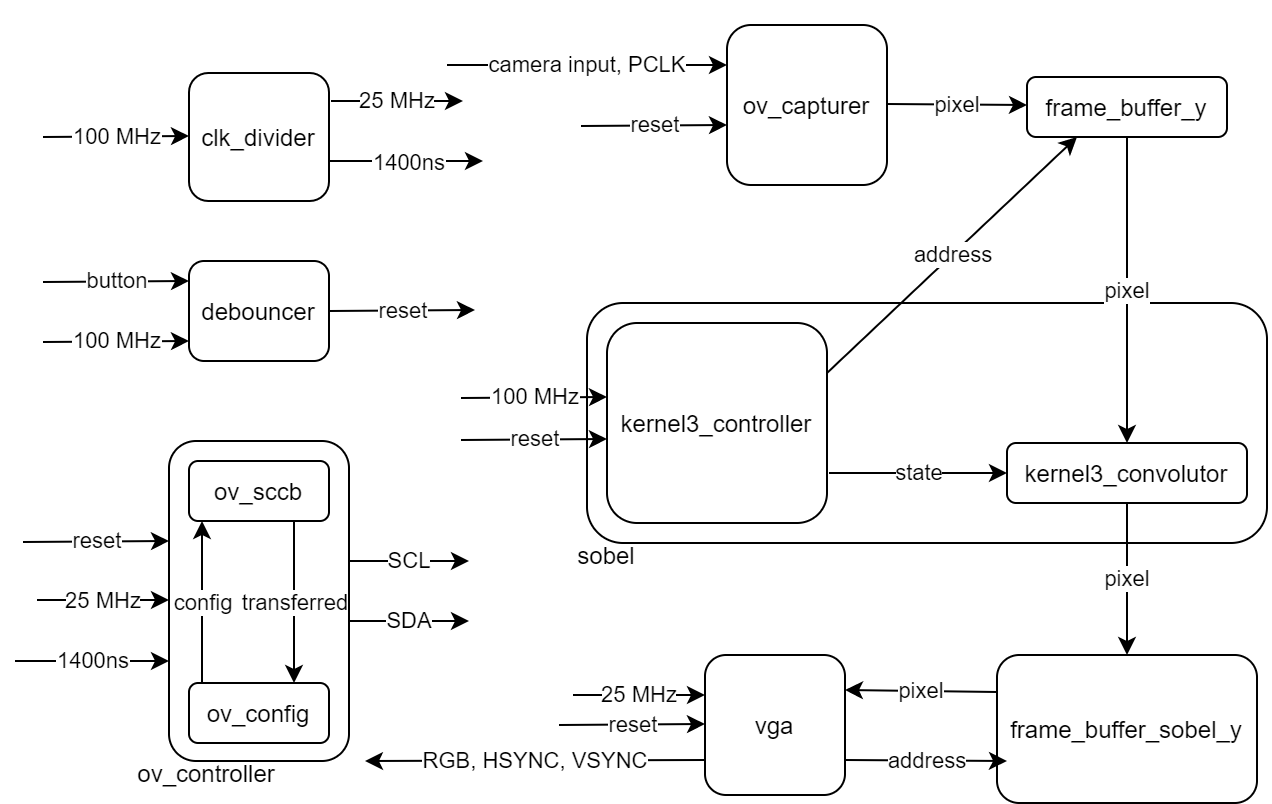
\includegraphics[scale=0.27]{block}
		\caption{Block Diagram}
		\label{fig:block}
	\end{figure}
	Fig. \ref{fig:block} shows the top level design of the current system. There are 10 components in total, including 2 frame buffers.
	\begin{enumerate}
		\item \texttt{clk\char`_divider} is responsible for taking a fast clock input, and generate a clock that is slower than the input by factors of multiples.
		\item \texttt{debouncer} is responsible for stabilizing button inputs. The output will only be 1 if the input has stayed 1 for a certain amount of time.
		\item \texttt{ov\char`_sccb} is responsible for configurating the camera. Without the configuration, the camera looks so bad, that one may be misled that the camera is faulty.
		\item \texttt{ov\char`_config} stores the values of the registers to be sent. Once \texttt{ov\char`_sccb} finishes sending a register, it notifies \texttt{ov\char`_config} to provide the next one, until all registers have been sent.
		\item \texttt{ov\char`_capturer} interfaces incoming data from the camera, and puts it into the first frame buffer \texttt{frame\char`_buffer\char`_y} (Y stands for the luma (brightness) component in the YUV color space).
		\item \texttt{kernel3\char`_controller} provides coordinates for each clock. These coordinates go to \texttt{frame\char`_buffer\char`_y}, and the returned pixel is fed to the \texttt{kernel3\char`_convolutor}.
		\item \texttt{kernel3\char`_convolutor} is running in synchronous to \texttt{kernel3\char`_controller}. For each clock cycle, it is supposed to receive a pixel in the 3x3 convolution matrix (the Sobel kernel for the current system), then do the multiplication with addition. Therefore, for every 9 cycles a pixel result should be formed. This result is fed to the next frame buffer (\texttt{frame\char`_buffer\char`_sobel\char`_y} for the current system).
		\item \texttt{vga} is responsible for generating the video output signal, by taking pixels from the last frame buffer.
	\end{enumerate}
	\section{Implementation Details}
	\begin{figure}[h]
		\centering
		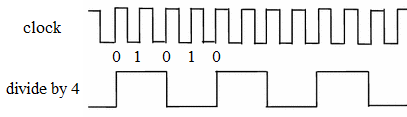
\includegraphics[scale=0.6]{clockdivider}
		\caption{The bottom clock toggles when the counter reaches 0}
		\label{fig:clockdivider}
	\end{figure}
	\texttt{clk\char`_divider} and \texttt{debouncer} are the easiest to implement. Both utilizes a counter. For \texttt{clk\char`_divider}, the counter is increased by one when there is a positive edge, and the output clock toggles if this counter has reached a particular threshold, illustrated in Fig. \ref{fig:clockdivider}. For \texttt{debouncer}, for each clock the state of the button is checked. The \texttt{debouncer} output will be 1 only if the button has been pressed for certain consecutive numbers of clock. \texttt{debouncer} is required because of the mechanical nature of the button, it tends to micro-vibrate when it is being pressed and released. The reset button is currently being wired to this \texttt{debouncer}, otherwise the reset will toggle between 0 and 1 constantly for a short burst, something that the camera cannot handle.
	
	\begin{figure}[h]
		\centering
		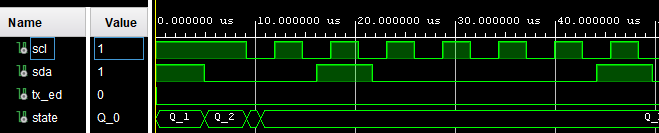
\includegraphics[scale=0.52]{sccb1}
		\caption{Start condition of SCCB. The first byte being transferred is 0x42, the SCCB address of OV7670}
		\label{fig:sccb1}
	\end{figure}
	\begin{figure}[h]
		\centering
		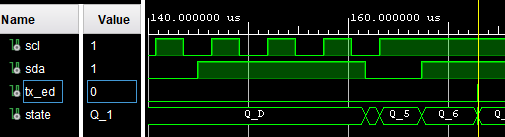
\includegraphics[scale=0.52]{sccb2}
		\caption{End condition of SCCB: SDA being pulled high while SCL is high}
		\label{fig:sccb2}
	\end{figure}
	
	\texttt{ov\char`_sccb} implements the SCCB protocol \cite{sccbdatasheet} published by OmniVision. It is very similar to the traditional I\textsuperscript{2}C protocol. One configuration transfer is broken up into 8 states (Fig. \ref{fig:sccb1} and \ref{fig:sccb2}), in which the SCL and SDA lines are toggled accordingly. \texttt{Q\char`_D} state is the data transfer state, which consists of 3 bytes, each 8 bits with 1 don’t-care bit. For I\textsuperscript{2}C, this don’t-care bit is supposed to be an acknowledgment, but for SCCB it should be pulled high-Z. To keep track of all these information, multiple counters are used, and state transitions are determined according to them when there is a clock edge.
	\begin{figure}[h]
		\centering
		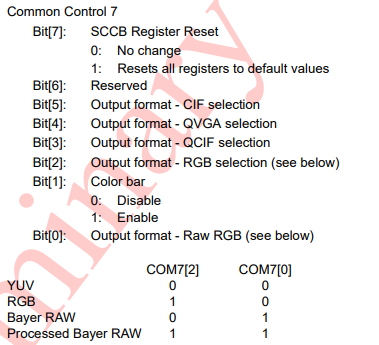
\includegraphics[scale=0.6]{com72}
		\caption{0x12 COM7}
		\label{fig:com72}
	\end{figure}
	\texttt{ov\char`_config} sends out register configurations one by one. There are 0xC9 registers from the data sheet. The most important register is 0x12 COM7 (the name of the register), shown in Fig. \ref{fig:com72}. With COM7, color mode between YUV and RGB565 can be toggled. The exact configuration has been copied from the Linux kernel, after understanding the C code \cite{reg6} and filtering out the registers that I need.
	\begin{figure}[h]
		\centering
		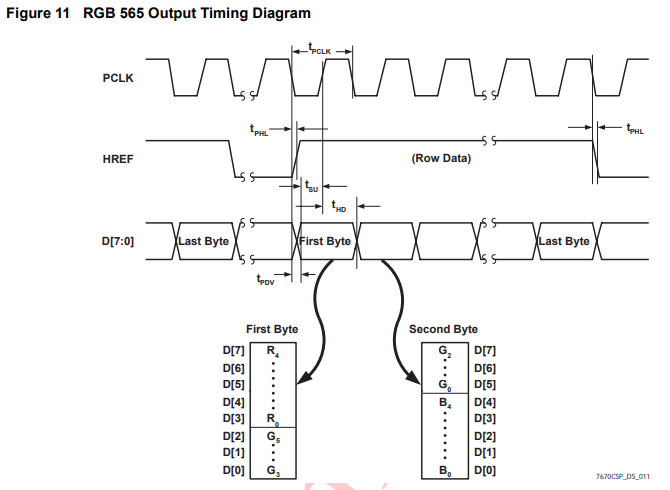
\includegraphics[scale=0.5]{rgb565}
		\caption{Waveform of pixel transfer}
		\label{fig:rgb565}
	\end{figure}
	\texttt{ov\char`_capturer} is purely passive, it responds to pixel clock from the camera. Each pixel is transferred in 2 clocks (Fig. \ref{fig:rgb565}), so a shift register is used to save the data from the first clock. The coordinate is incremented roughly every 2 clocks (roughly because there is no data transfer for line increments), until the whole frame is refreshed. For every pixel, the capturer writes it to the first buffer (\texttt{frame\char`_buffer\char`_y}).
	
	\texttt{kernel3\char`_controller} shifts coordinates every 9 clocks. Within these 9 clocks, it visits the 8-neighbor, and itself, from left to right, top to bottom. There are border detections, that if a neighbor goes out of bound, the output coordinate becomes the starting pixel itself. Each pixel from the camera arrives every 2 cycles, but for this controller it needs to consider 9 times more pixels. Luckily the controller is separated from the camera, it can be fed with the fastest clock available from the ZedBoard (100 MHz), with a frame buffer in between. That’s why the first frame buffer exists. Even if the clocks are in the same frequency, the buffer is still needed because the clocks may not be in phase, since one of them is from an external source.
	
	\texttt{kernel3\char`_controller} gives the address to the first buffer, the buffer returns the pixel value to \texttt{kernel3\char`_convolutor}. The controller also sends a state number to convolutor, so that the convolutor knows which matrix entry it should multiply the pixel with. For every 9 cycles, a pixel’s calculation has been finished, and the result is written to the second buffer (\texttt{frame\char`_buffer\char`_sobel\char`_y}). In the current system, 2 convolutor instances are fed with the Sobel kernels \cite{sobel}
	\begin{align*}
		G_x&=
		\begin{pmatrix}
			1&0&-1\\
			2&0&-2\\
			1&0&-1
		\end{pmatrix},\\
		G_y&=
		\begin{pmatrix}
			1&2&1\\
			0&0&0\\
			-1&-2&-1
		\end{pmatrix}.
	\end{align*}
	
	There is some glue code between the controller and the convolutor. Specifically, 2 \texttt{kernel3\char`_convolutor}s have been instantiated, one for x and one for y. Technically, the two resultant values should be squared, added together then taken the square root
	\begin{align*}
		G&=\sqrt{{G_x}^2+{G_y}^2}
	\end{align*}
	. Since the maximum value of $G_x$ and $G_y$ can be 4 times of the maximum pixel value, the initial implementation divides the result by 4, which is technically incorrect. The correct way is to leave the result as is, then bound the result if it exceeds the minimum or the maximum. In the current implementation, $G_x$ and $G_y$ are averaged, since this is easier to implement while still being reasonable. The original bound is not mathematically rigorous anyway. However, this resulted in an almost black screen, since the resulted values were too small after being divided by 4. Originally, the bounding method was then tested, but it produced so much noise (fig. \ref{fig:real1}) due the quality of the camera\begin{figure}[h]
		\centering
		\includegraphics[scale=0.095]{real1}
		\caption{Very noisy}
		\label{fig:real1}
	\end{figure}. This was verified by pointing the camera to a blank paper, where purple dots (fig. \ref{fig:real2}, \ref{real3}) can be seen.
\begin{figure}[h]
		\centering
		\includegraphics[scale=0.052]{real2}
		\caption{Purple dots despite shooting at a blank paper}
		\label{fig:real2}
	\end{figure}
\begin{figure}[h]
		\centering
		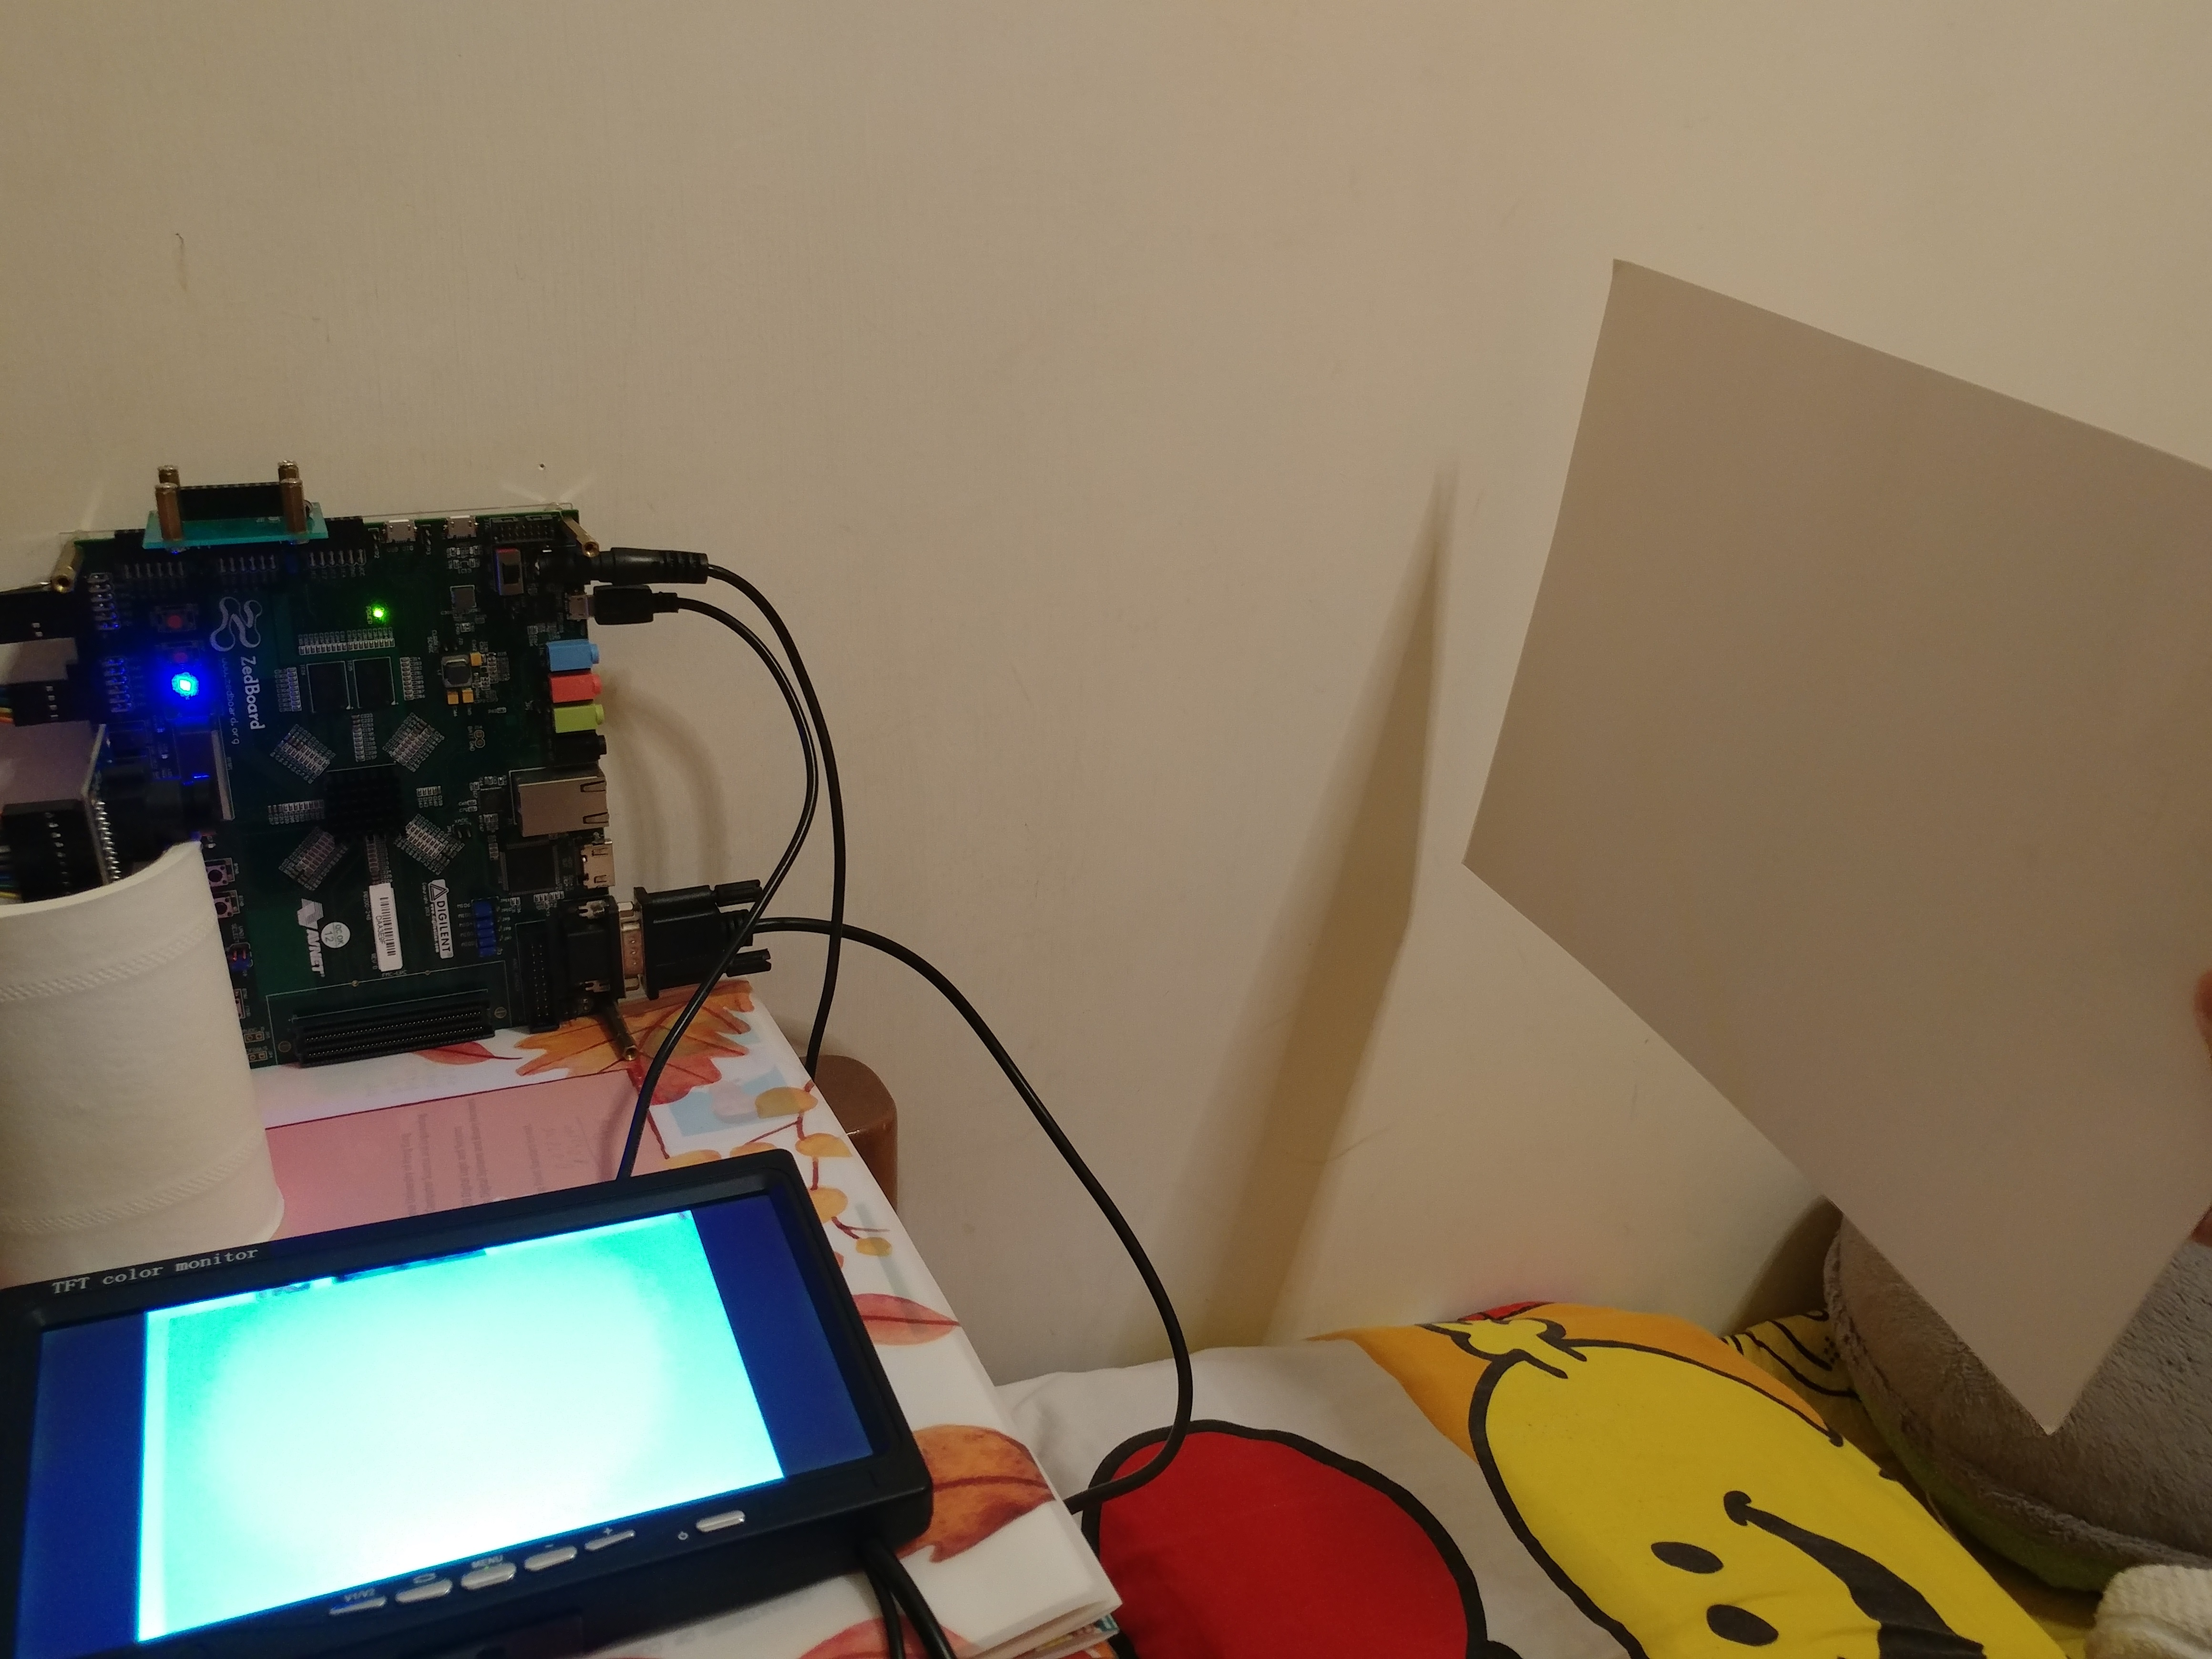
\includegraphics[scale=0.052]{real3}
		\caption{It is indeed the white paper}
		\label{fig:real3}
	\end{figure}
To deal with this, the Gaussian blur filter 3x3 
	\begin{align*}
		\frac{1}{16}
		\begin{pmatrix}
			1&2&1\\
			2&4&2\\
			1&2&1
		\end{pmatrix}
	\end{align*}
	was tried, unfortunately it made no difference.
	The current implementation mixes both the correct and incorrect approaches, by first taking the absolute value, then dividing, multiplying back, and the final result is then bounded. Take $G_x$ as an example:
	\begin{align*}
		G_x&=\text{bound}\left(4\left\lfloor{ \frac{1}{4}\left |
		\begin{pmatrix}
			1&0&-1\\
			2&0&-2\\
			1&0&-1
		\end{pmatrix}\right|} \right\rfloor
		\right).
	\end{align*}
	 This implementation removes all the noise, because of the division (implemented as shifts) making them zero. However, some tiny portions of the supposedly edges are also lost in this process (fig. \ref{fig:real4}).
\begin{figure}[h]
		\centering
		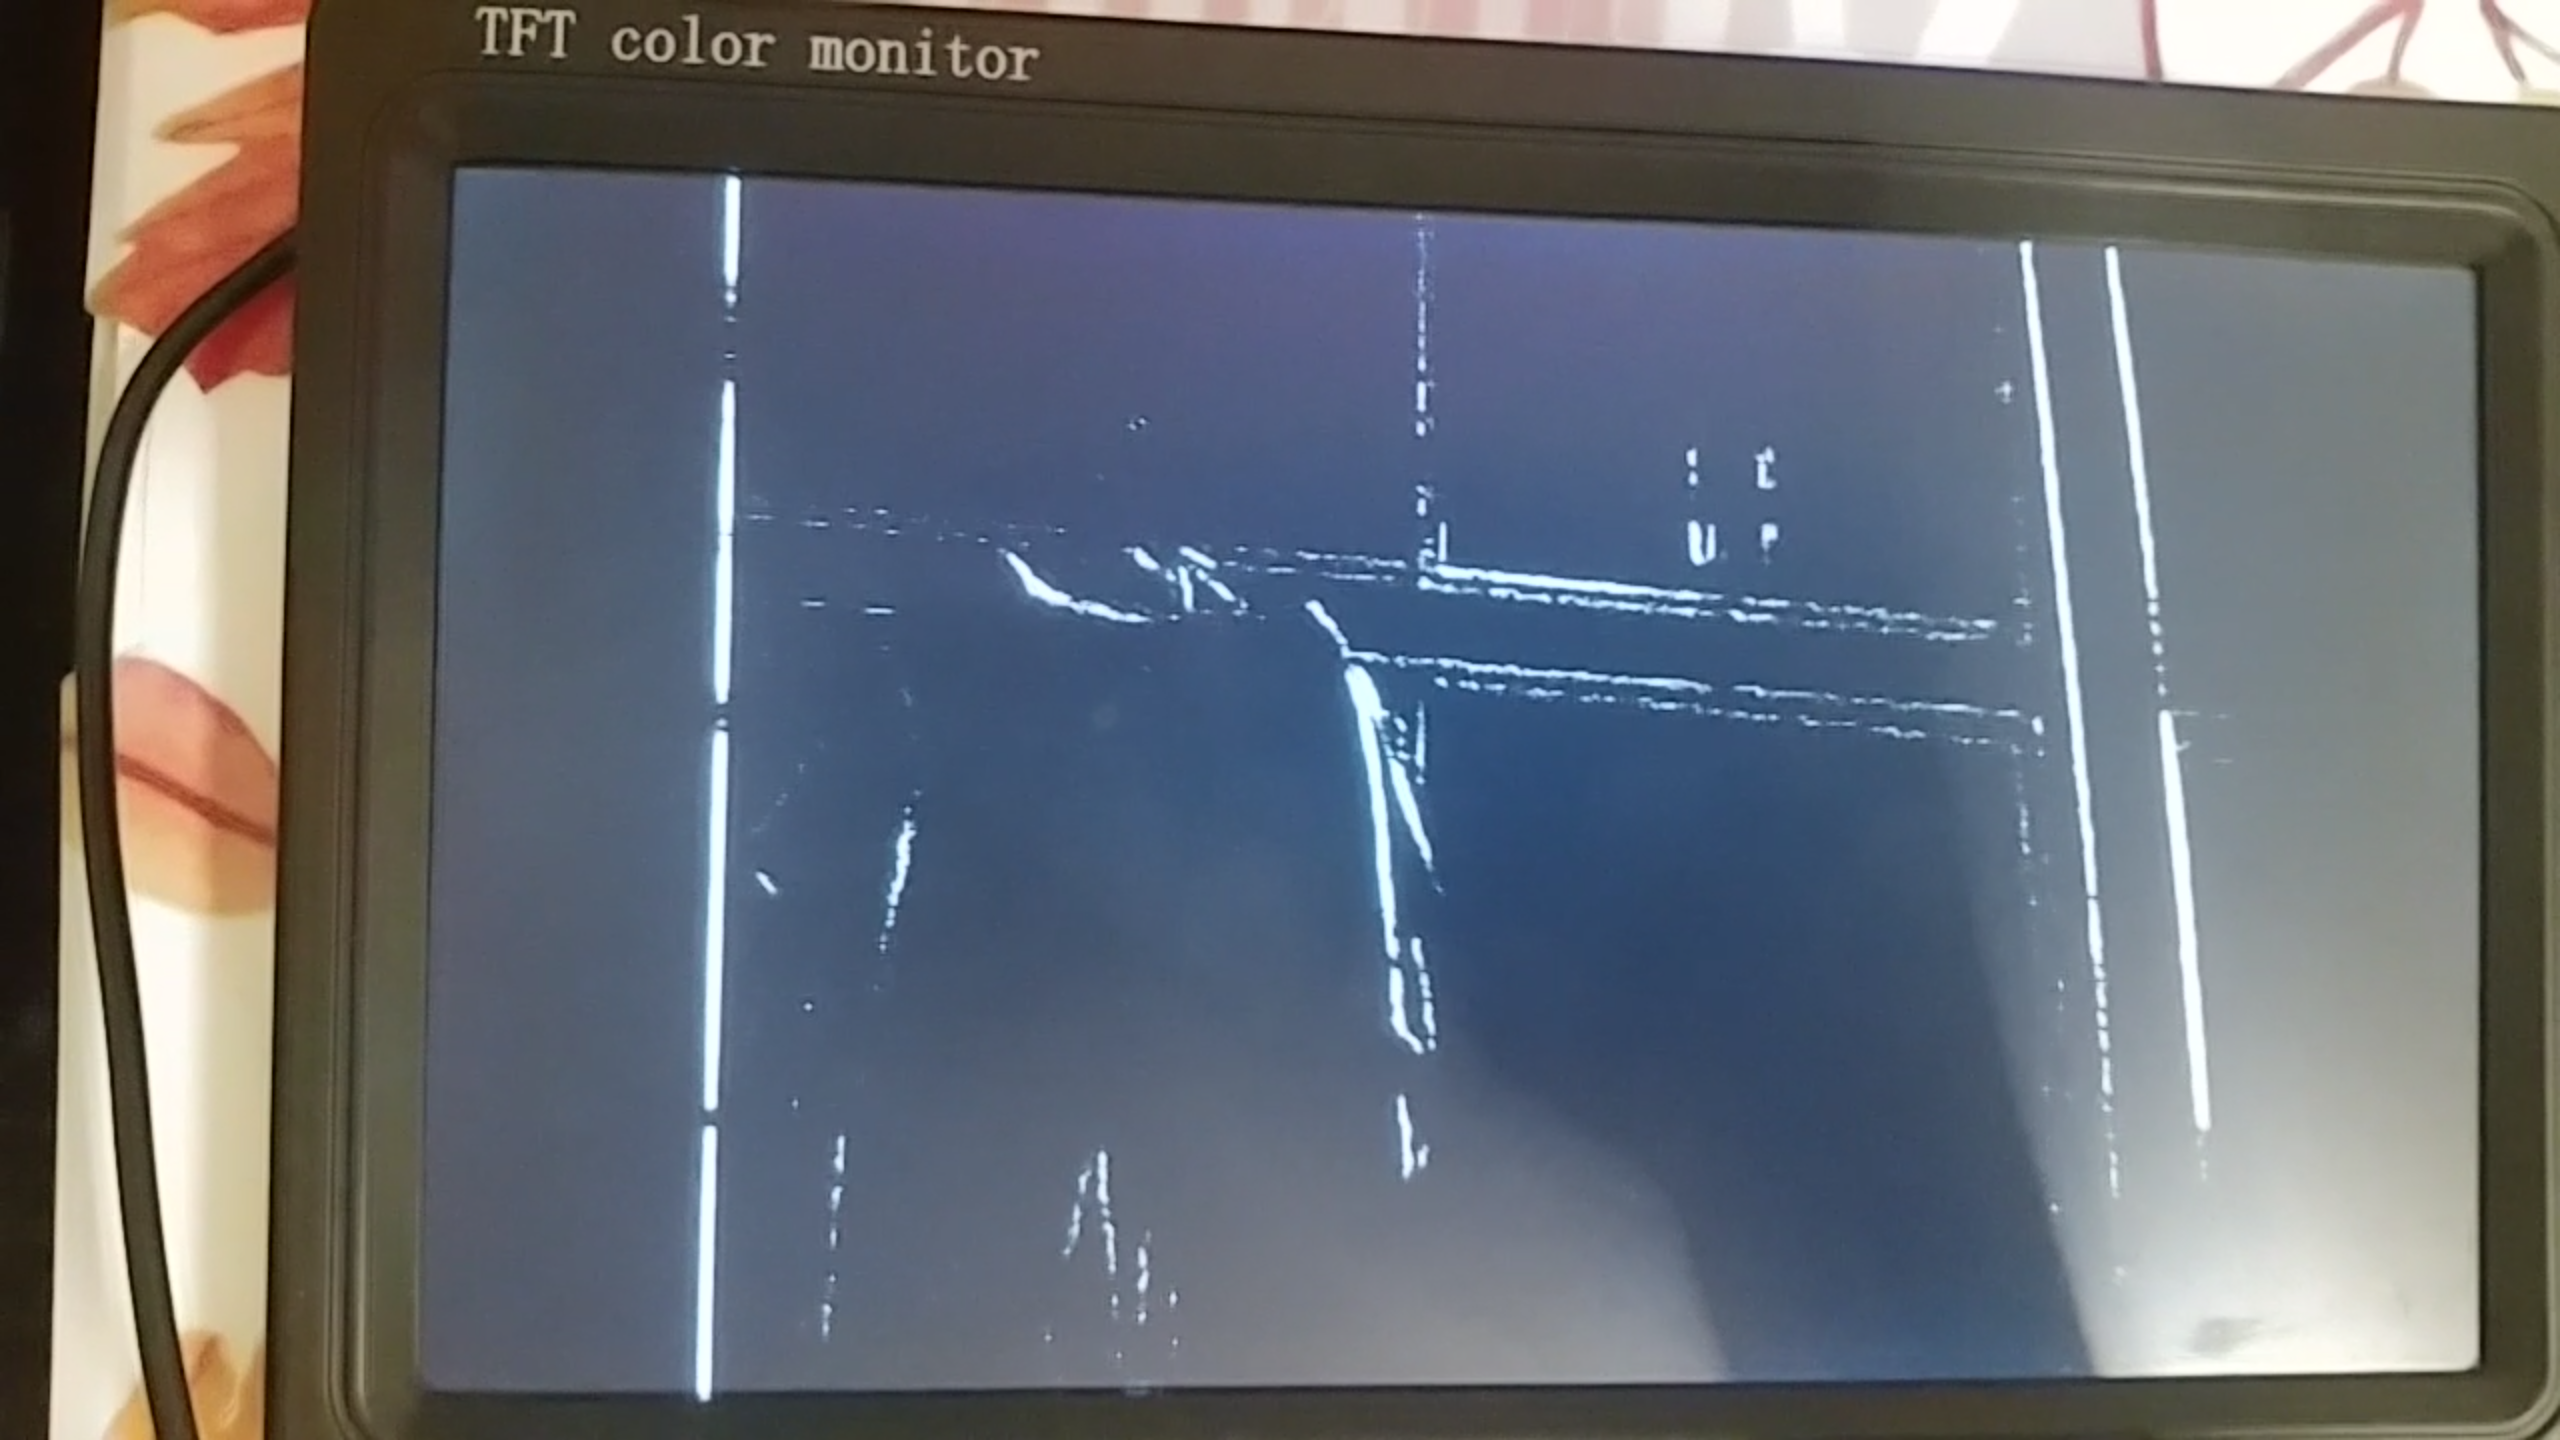
\includegraphics[scale=0.095]{real4}
		\caption{Some edges lost}
		\label{fig:real4}
	\end{figure}
	 This result comes from the fact that the camera cannot produce highly distinct colors for real edges. If the camera is fed by black and white 2D codes, which is the main use case for robots, the edges are very clean (fig. \ref{fig:real5}, \ref{fig:real6}).
\begin{figure}[h]
		\centering
		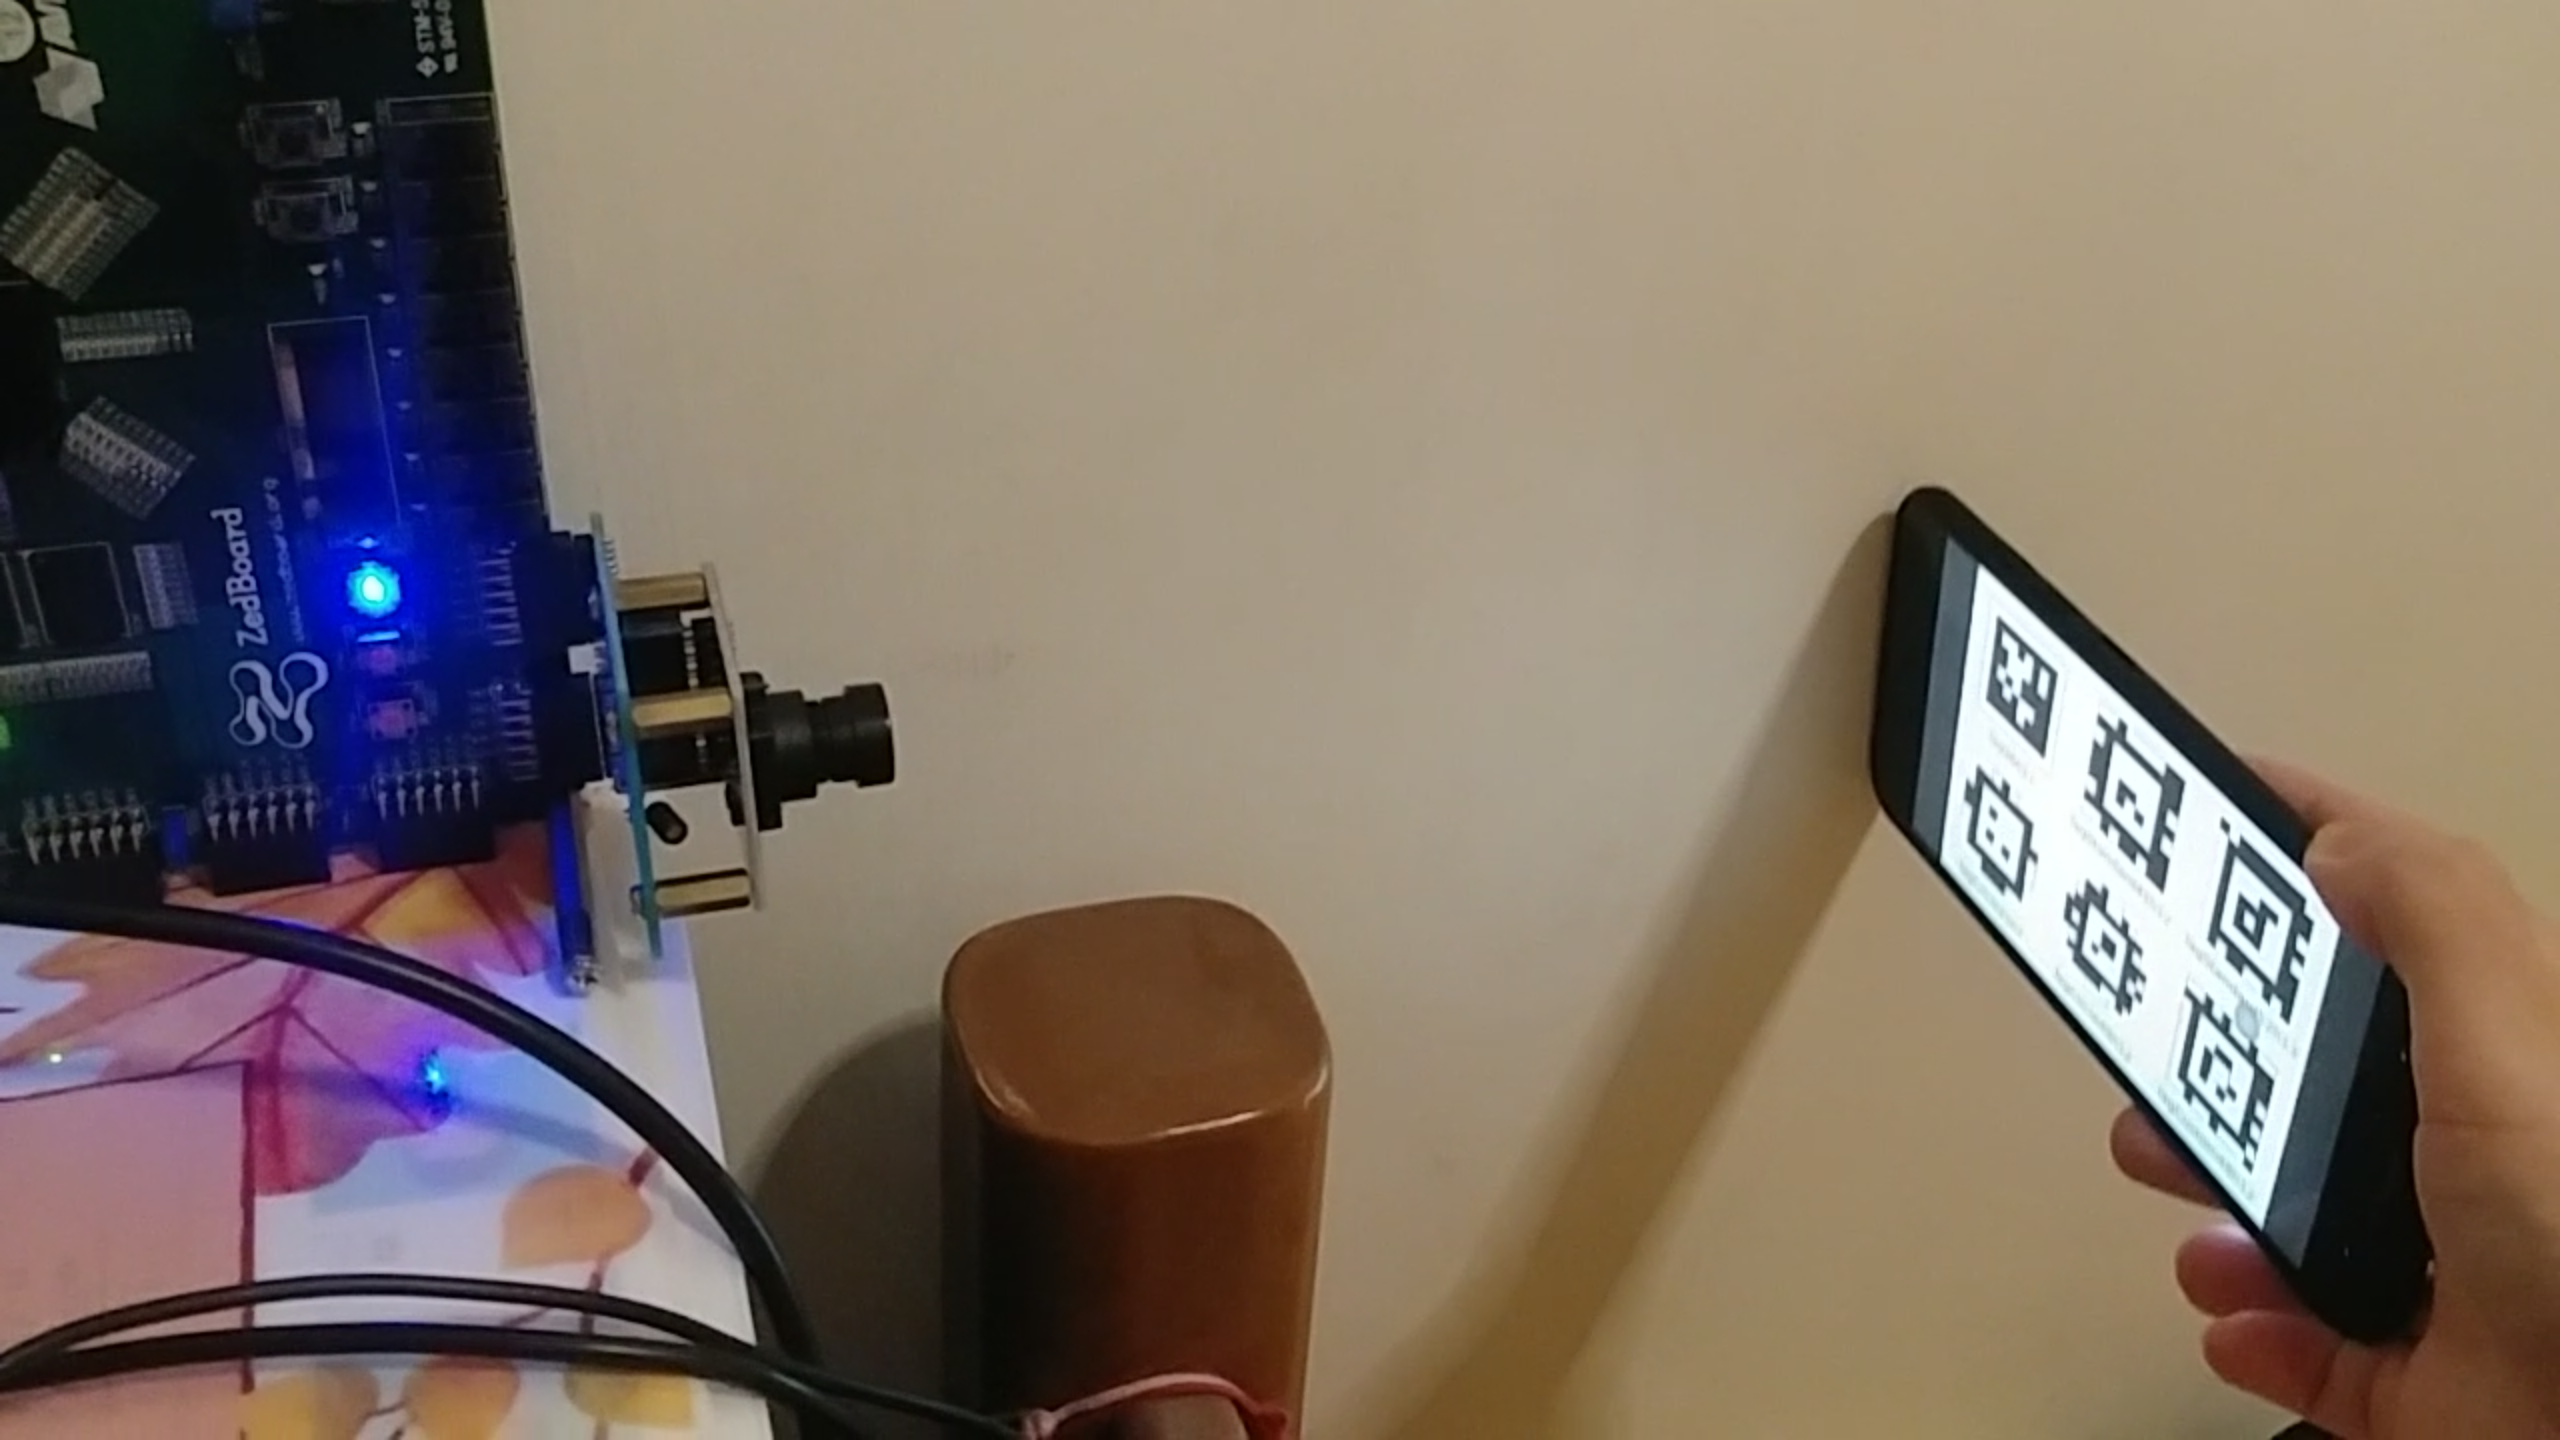
\includegraphics[scale=0.095]{real5}
		\caption{AprilTags}
		\label{fig:real5}
	\end{figure}
\begin{figure}[h]
		\centering
		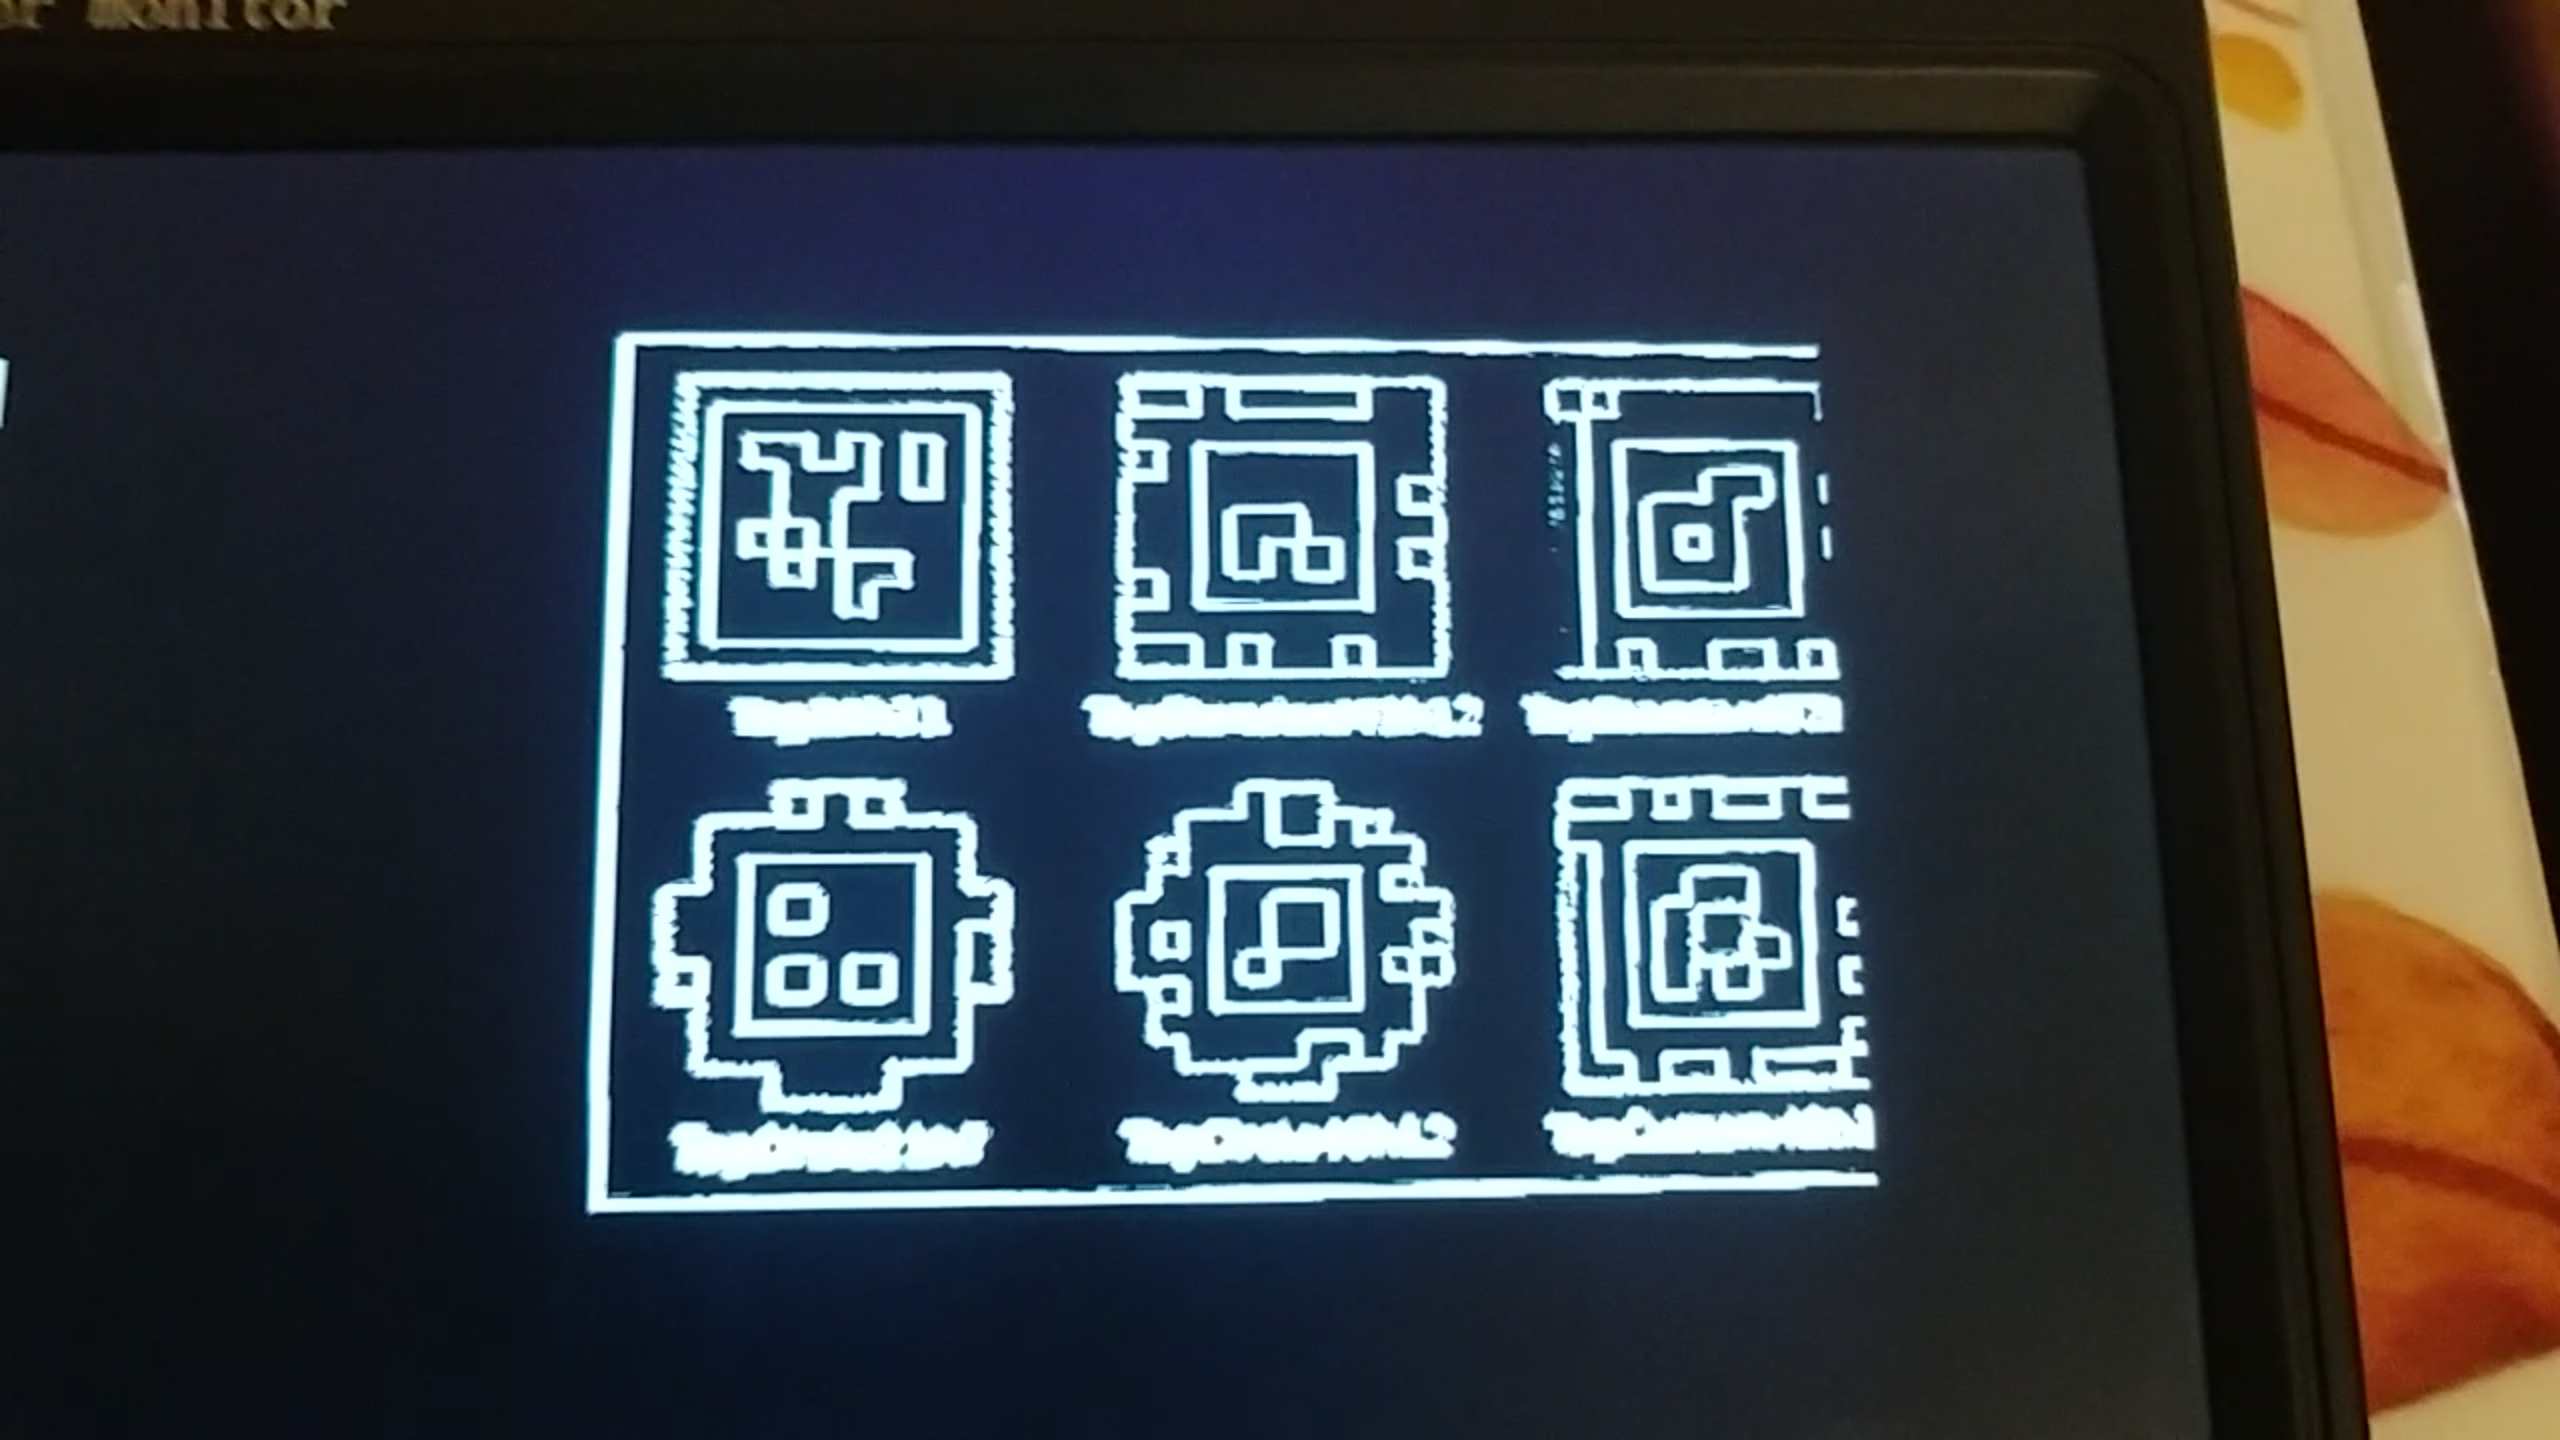
\includegraphics[scale=0.095]{real6}
		\caption{Clean output}
		\label{fig:real6}
	\end{figure}
	
	Finally, \texttt{vga} pulls data from the second buffer, and output the appropriate video signals.
	
	The camera’s SCCB runs at a period of 5600 ns. The camera runs at 25 MHz, the convolution runs at 100 MHz, and standard VGA runs at 25 MHz.
	\section{Difficulties}
	A huge amount of time has been spent on dealing with the camera. The main problem comes from the poor quality of the data sheet. Before getting hands on the camera, I thought the camera would either 1) work, and produces ideal/usable frames, or 2) produce no output at all. Obviously, now I know how wrong I was. There are numerous registers sets \cite{reg1}\cite{reg2}\cite{reg3}\cite{reg4}\cite{reg5} for the OV7670, but none of them works perfectly (at least to the current extent) on the ZedBoard. Most of them contradict with each other, probably due to different units which the camera are being controlled from. Some configurations do work (have a video output), but they either have weird colors and white balance, or unbearable noise levels. I tried fixing the configurations on my own, but there are many camera-specific abbreviations on the data sheet that I could not understand. There are also just too many registers.
	
	Finally, the Linux set of configurations \cite{reg6} were found and adapted. Even that did not work on the FPGA initially, but the artifacts were sorted out eventually. Comments from the Linux kernel source code \cite{reg6} have been encouraging though: 
	\begin{displayquote}
		\textbf{Line 200}: (the registers) do not always make complete sense to humans\\
		\textbf{Line 384}: Extra-weird stuff\\
		\textbf{Line 1045}: a pain in the \_\_\_\\
		\textbf{Line 1289}: Weird crap\\
		\textbf{Line 1466}: If one believes the data sheet, …
	\end{displayquote}
	So at least someone else in the world had been sharing the same frustration as me.
	
	Apart from the problems documented in the kernel code, another problem I find is that if COM7 is sent 0x80 (soft reset) 3 times in a row, the camera will pass out immediately. If only one COM7 command is sent out, it likely still will not work, due to the camera needing a settling time of 1 ms. That is why hardware reset is being used, controlled by a button with debouncing. Normally a button will be pressed for longer than 1 ms.
	
	Another notable data sheet bug is, if the SCCB runs well below the maximum frequency 400 KHz, i.e., well above minimum period 2500 ns, stated in the data sheet, at 2800 ns, the camera will flicker. The current implemented SCCB speed runs at 5600 ns.
	
	To make matters worse, this camera sensor by itself has high variations. The first sensor that I borrowed from the laboratory straight up did not work. The second did work but was not great, and it was not until the third one which has been bearable. Before that, whenever there was a problem, I could not tell if the problem was from my logic, from the configurations, or from the camera.
	
	When it comes to difficulties not related to the camera, it mainly has to do with me being a newbie in hardware coding. I have to think in clock cycles, instead of sequential instructions, which is not something I have been used to. VHDL’s syntax being new to me does not help either. Even though I have heard VGA and I\textsuperscript{2}C before, I did not know how they work. In the end, everything has been rewritten, because I could not figure out how to remove problems from code segments found online. Which  means that now I know how the protocols work. If I had taken the computer engineering course about FPGAs, these stuff may have been solved quicker.
	
	A few testbenches have been written to verify the code, but they have only been for stuff that I know how to test. I did not know how to test bugs related to the camera, or frame buffers. For example, the convolution module has been written in less than two days, but for a long time the video output has been blank (it turned out to be yet again, some problems related to the camera), and I got confused.
	
	In terms of logistic difficulties, they were relatively minor. Back in May, I borrowed another FPGA evaluation board ZCU102. Although it is more powerful, it lacks basic I/O that I need, such as VGA. Eventually I returned it, and settled for the ZedBoard.
	
	Then, for the first few weeks of the semester, I needed to go back to the laboratory because I did not realize VGA monitor can be borrowed. When I was at home, I read how QR codes \cite{utube1}, DataMatrices\cite{utube2} and AprilTags are decoded \cite{apriltag}\cite{apriltag2}, and also how certain algorithms can be implemented on FPGAs. Some ideas of FPGA algorithms to detect these codes have also been appearing in my mind. But the implementation side of things have been lagging behind. Long compilation and synthesis time from Vivado also contributed to the slow implementation progress (fig. \ref{fig:vivado}). It is a lot longer than what I am used to, being able to compile software code in a minute.
	\begin{figure}[h]
		\centering
		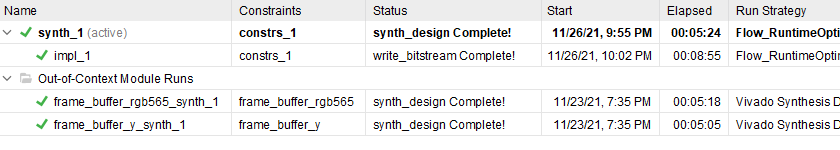
\includegraphics[scale=0.4]{vivado}
		\caption{A single Vivado synthesis takes 14 mins}
		\label{fig:vivado}
	\end{figure}
	\section{Future Work}
	The most immediate target is to ease debugging. A new testbench should be written, such that it takes a picture file from the computer, process the file with the HDL modules, and write the file back to disk. This way, slow synthesis can be avoided more often.
	
	The second target is to figure out how to store the frame buffer on the on-board DRAM. Right now, frame buffers are on block RAM, but block RAM on this SoC is rather limited. It is not sure at this point, if the DRAM is wired to the FPGA, or it is just limited to the processing system.
	
	FPGA techniques and algorithms should be the focus of the next semester. Traditional sequential algorithms, such as finding the trigonometry function of a floating point number, or finding a patch of similar pixels with BFS or DFS, cannot be easily implemented on FPGAs. A few techniques, namely connected component analysis \cite{cca} and CORDIC have been found, and may be useful (and difficult).
	
	Also, hopefully a way to generate the whole Vivado project using a single Tcl script will be figured out. Vivado generates a lot of cache files, and they are not being friendly to the version control system. Currently, the whole project directory is being tracked, with only primitive git ignore files.
	
	Lastly, a VGA library to output text and basic graphics will be nice and interesting, if it can be found online or written on my own. Depending on the actual benefits, for example its usefulness on debugging, this may be skipped.
	\section{Conclusion}
	A complete system with Sobel edge detection has been developed in VHDL, as a baseline for further algorithmic development. Lots of hardware problems have been solved, and should no longer be encountered.
	\newpage
	\begin{thebibliography}{99}
        \bibitem{vga}
            MIT 6.111 Lab Kit: \textit{VGA Video}, \begin{verbatim}https://web.mit.edu/6.111/www/s2004/NEWKIT/vga.shtml\end{verbatim}
            
        \bibitem{rpi}
            Joshua Hrisko: \textit{Image Processing Object Detection with Raspberry Pi and Python}, \begin{verbatim}https://makersportal.com/blog/2019/4/23/image-processing-with-raspberry-pi-and-python-part-ii-spatial-statistics-and-correlations\end{verbatim}            
            
	\bibitem{ovdatasheet}
	OV7670 Data Sheet \begin{verbatim}http://web.mit.edu/6.111/www/f2016/tools/OV7670_2006.pdf\end{verbatim}
	\bibitem{sccbdatasheet}
	SCCB Reference\begin{verbatim}https://www.waveshare.com/w/upload/1/14/OmniVision_Technologies_Seril_Camera_Control_Bus\%28SCCB\%29_Specification.pdf\end{verbatim}
	
	\bibitem{sobel}
	Wikipedia: \textit{Sobel Operator}\begin{verbatim}https://en.wikipedia.org/wiki/Sobel_operator\end{verbatim}
    
	\bibitem{utube1}
	How to Decode a QR Code by Hand: \begin{verbatim}https://www.youtube.com/watch?v=KA8hDldvfv0\end{verbatim}
	\bibitem{utube2}
	How to Decode a DataMatrix Code by Hand: \begin{verbatim}https://www.youtube.com/watch?v=w0xVd2xXySo\end{verbatim}
	\bibitem{apriltag}
	Edwin Olson: \textit{AprilTag: A robust and flexible visual fiducial system}\begin{verbatim}https://april.eecs.umich.edu/media/pdfs/olson2011tags.pdf\end{verbatim}
    
	\bibitem{apriltag2}
	Ethan Tola: \textit{Real-Time UAV Pose Estimation and Tracking using FPGA Accelerated April Tag}\begin{verbatim}https://scholarworks.rit.edu/cgi/viewcontent.cgi?article=11999&context=theses\end{verbatim}
	
	\bibitem{cca}
	D.G. Bailey, C.T. Johnston: \textit{Single Pass Connected Components Analysis}\begin{verbatim}http://sprg.massey.ac.nz/pdfs/2007_ivcnz_282.pdf\end{verbatim}
	
	
	\bibitem{reg1}
	Register Set 1: \begin{verbatim}https://web.archive.org/web/20150402065629/http://hamsterworks.co.nz/mediawiki/index.php/Zedboard_OV7670\end{verbatim}
	\bibitem{reg2}
	Register Set 2: \begin{verbatim}https://github.com/jonlwowski012/OV7670_NEXYS4_Verilog/blob/master/ov7670_registers_verilog.v\end{verbatim}
	\bibitem{reg3}
	Register Set 3: \begin{verbatim}https://github.com/iwatake2222/DigitalCamera_STM32/blob/master/Src/driver/ov7670/ov7670Reg.h\end{verbatim}
	\bibitem{reg4}
	Register Set 4: \begin{verbatim}https://92zo.at.webry.info/201301/article_2.html\end{verbatim}
	\bibitem{reg5}
	Register Set 5: \begin{verbatim}https://github.com/adafruit/Adafruit_OV7670/blob/master/src/ov7670.c\end{verbatim}
	\bibitem{reg6}
	Register Set 6: \begin{verbatim}https://github.com/torvalds/linux/blob/master/drivers/media/i2c/ov7670.c\end{verbatim}
	
	
    \end{thebibliography}
\end{document}
